
%% ================================================================
%%  3.  BENCHMARKING ENVIRONMENT
%% ================================================================
\section{Benchmarking Environment}\label{sec:env}

Our benchmarking framework is built upon the
\texttt{or-gym}~\citep{hubbs2020orgym} inventory management environment,
which we modernize and substantially extend. The original OR-Gym
environment provided a Gymnasium-compatible simulation of multi-echelon
inventory networks with stationary Poisson demand and fixed cost
structures, using the now-deprecated OpenAI~Gym API.

Our extensions include: (i)~migration to the current
Gymnasium~API~\citep{brockman2016openai} with full compatibility with
Stable-Baselines3~\citep{raffin2021stable};
(ii)~composable, non-stationary demand patterns;
(iii)~endogenous goodwill dynamics that create demand--service feedback
loops; and (iv)~configurable network topologies ranging from single-node
to arbitrary directed acyclic graphs.

\subsection{Network Topologies}

The environment supports configurable directed acyclic graphs (DAGs)
representing multi-echelon supply chains. Each node
$n \in \mathcal{N}$ represents a facility (factory, distributor, or
retailer) with parameters:
\begin{itemize}
  \item $I_0^n$: initial on-hand inventory,
  \item $h_n$: per-unit holding cost per period,
  \item $C_n$: production or storage capacity,
  \item $p_n$: sale price (retail) or transfer price (intermediate).
\end{itemize}

Each directed edge $(i,j) \in \mathcal{E}$ has lead time $L_{ij}$ and
per-unit pipeline holding cost $g_{ij}$. The graph structure, cost
parameters, and lead times are fully configurable through a Python
dictionary, enabling researchers to define custom topologies.

We study two canonical topologies (\Cref{fig:topologies}):

\begin{enumerate}
  \item \textbf{Base (4-echelon distribution network):} A single
        raw-material supplier feeds two factories, which supply two
        distributors, which serve a single retailer. This creates a
        convergent network with 8~nodes and 7~edges, representative of
        distribution systems found in practice.

  \item \textbf{Serial (4-echelon chain):} A linear chain of 4~nodes
        (supplier $\to$ factory $\to$ distributor $\to$ retailer) with
        a single path. This is the classical Clark--Scarf
        topology~\citep{clark1960optimal}, for which optimal echelon
        base-stock policies are known under stationary demand, providing
        a theoretical baseline for comparison.
\end{enumerate}

The environment can also be configured as a single-node system,
reducing to a classical newsvendor problem---the simplest inventory
setting. This demonstrates the framework's generality: it spans the
full spectrum from single-item to complex multi-echelon networks.

\begin{figure}[htbp]
  \centering
  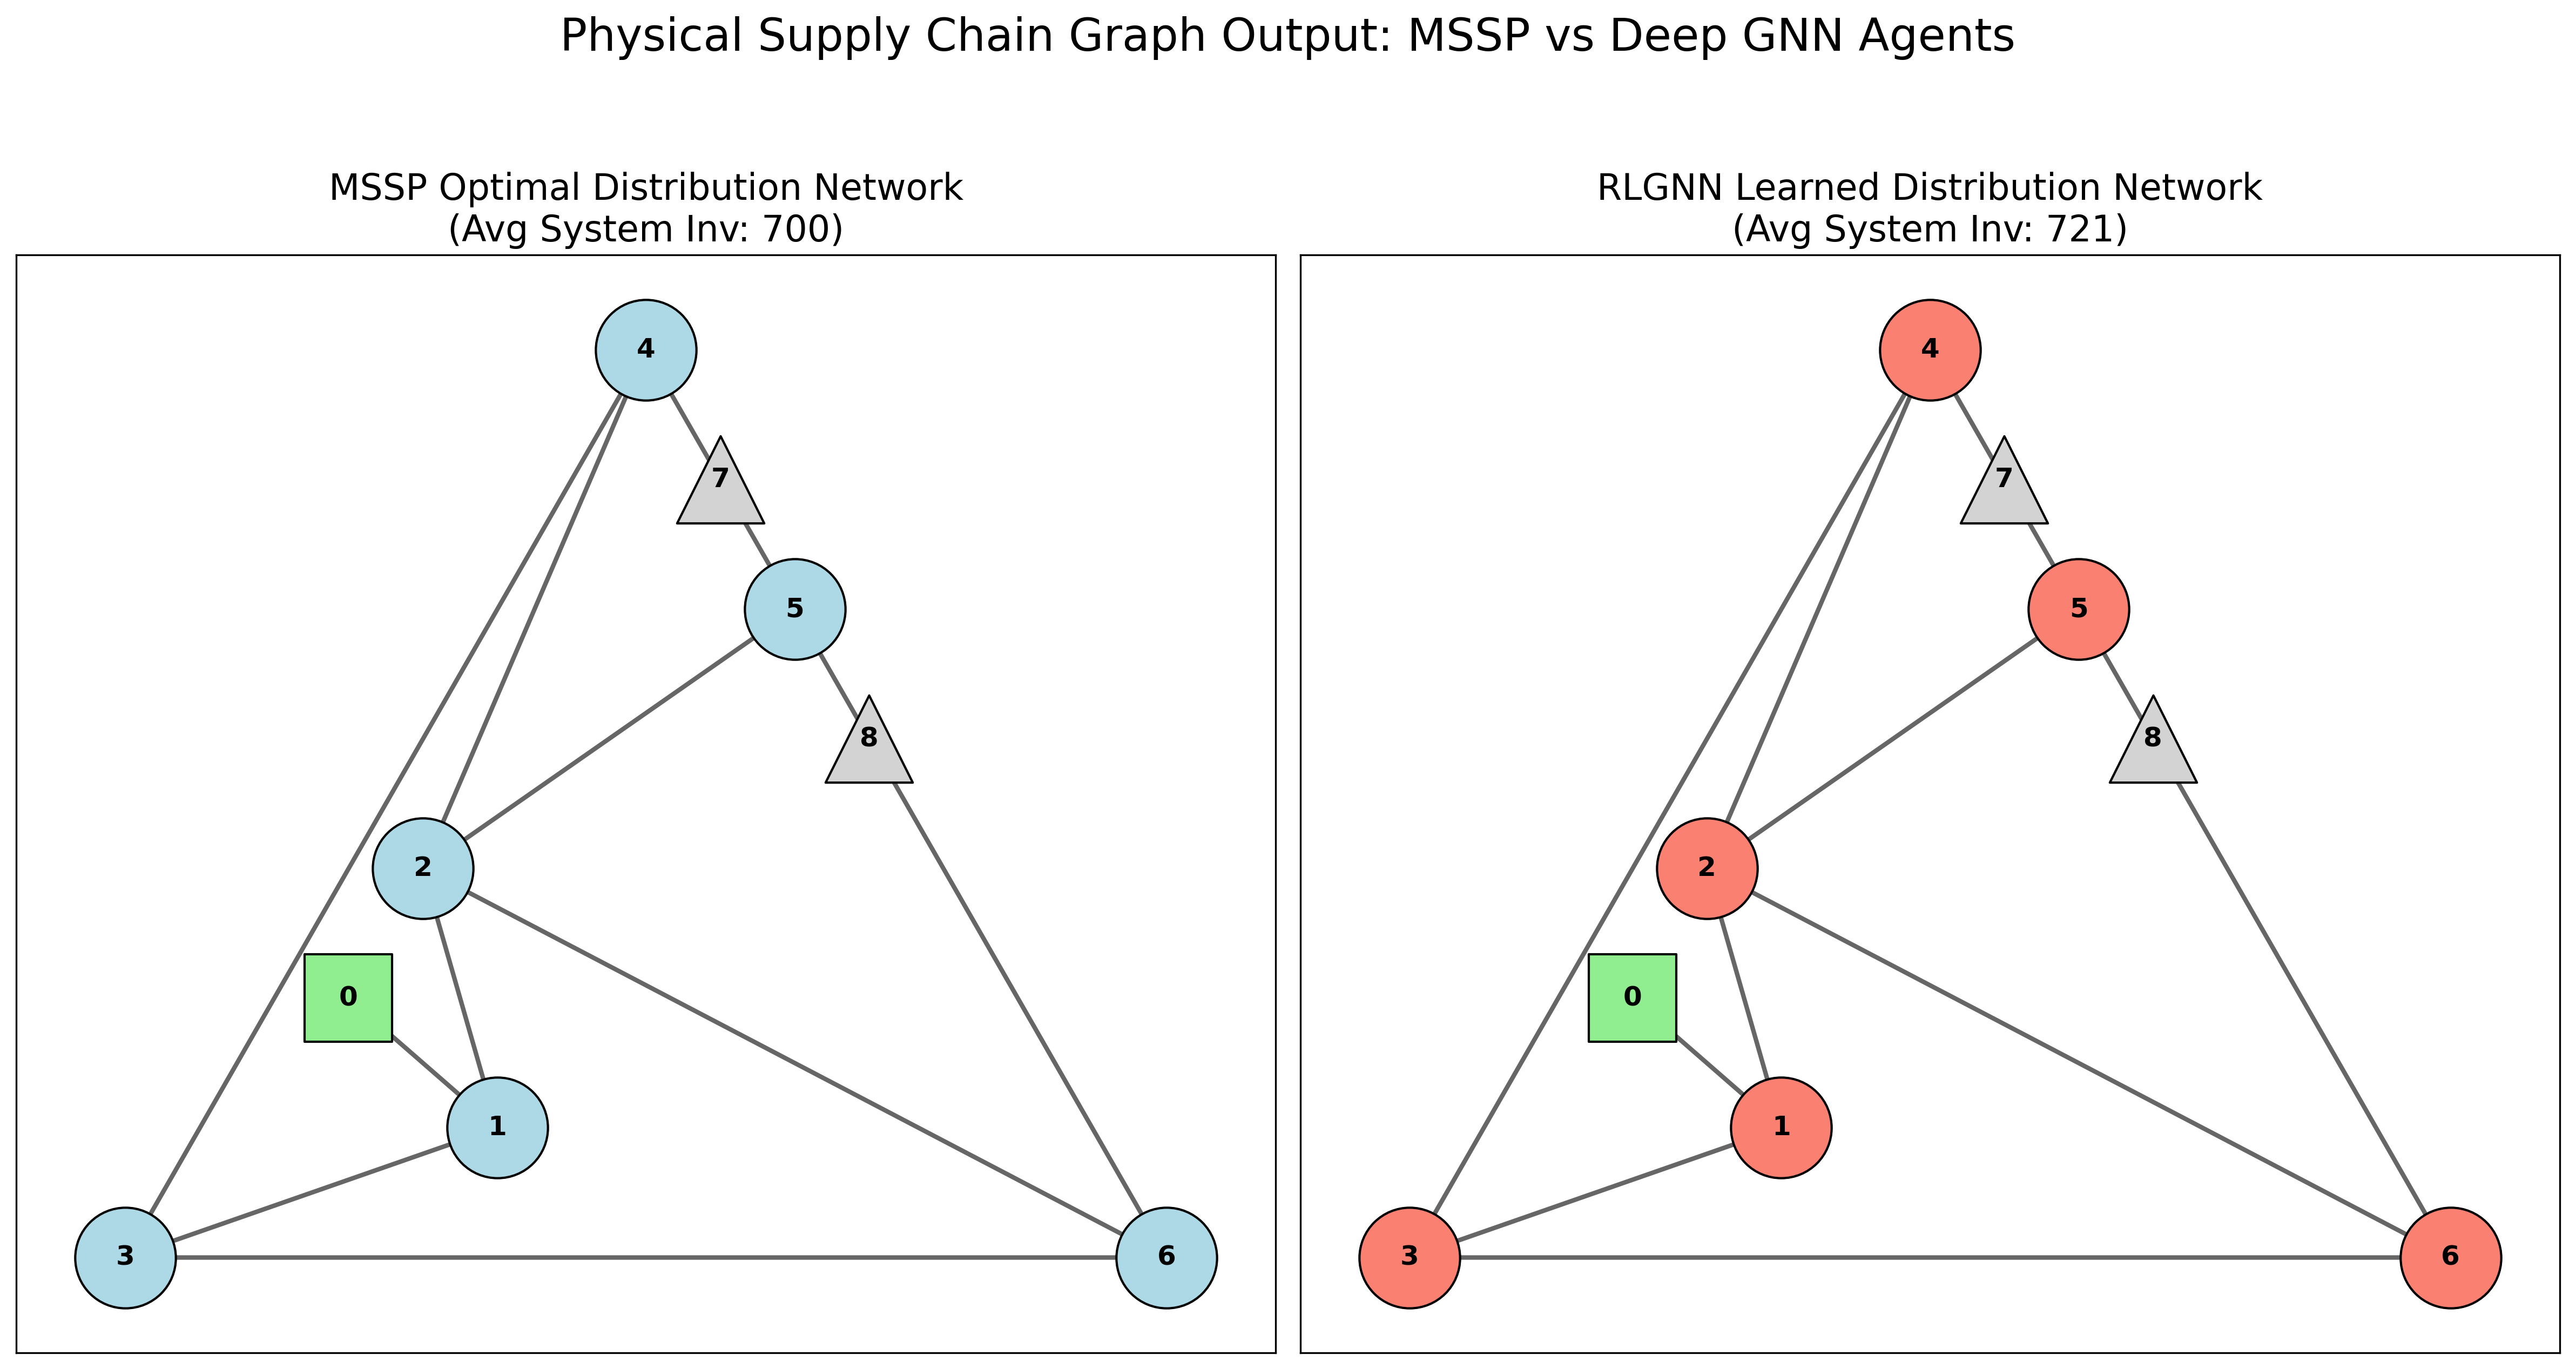
\includegraphics[width=0.9\textwidth]{figures/E_Network_Topology_Mapping.png}
  \caption{Network topologies used in the benchmark. \textbf{Left:}
           Base 4-echelon distribution network with convergent structure.
           \textbf{Right:} Serial 4-echelon chain (Clark--Scarf topology).}
  \label{fig:topologies}
\end{figure}

\subsection{Demand Patterns}\label{sec:demand}

A key extension over the original OR-Gym is our system of
\emph{composable demand patterns}. Customer demand $D_t$ at the retail
node is sampled from a Poisson distribution with time-varying mean
$\mu_t$. Starting from a base mean $\mu_0 = 20$, effects are applied
\emph{multiplicatively}, allowing patterns to be composed (e.g.,
seasonal~+~trend). We implement four demand patterns:

\begin{enumerate}
  \item \textbf{Stationary:} $\mu_t = \mu_0 = 20 \;\forall\; t$.
        This is the classical setting studied by
        \citet{clark1960optimal}, where OR methods have optimal or
        near-optimal theoretical guarantees.

  \item \textbf{Trend:} $\mu_t = \mu_0 \cdot (1 + \beta \cdot t)$
        with slope $\beta = 0.05$, creating a linearly increasing
        demand that approximately doubles over the 30-period horizon.
        This pattern tests an agent's ability to track systematic
        demand growth.

  \item \textbf{Seasonal:}
        $\mu_t = \mu_0 \cdot (1 + A \sin(\omega t))$,
        with amplitude $A = 0.5$ (50\% fluctuation) and angular
        frequency $\omega = 2\pi / 30$ (one full cycle per episode).
        This pattern tests responsiveness to predictable but
        time-varying demand.

  \item \textbf{Shock:} $\mu_t = \mu_0$ for $t < \tau$;
        $\mu_t = \mu_0 \cdot k$ for $t \geq \tau$, modelling an
        abrupt demand spike with $\tau = 15$ (mid-horizon) and
        multiplier $k = 2.0$ (demand doubles). This is the most
        challenging pattern for methods relying on distributional
        stationarity assumptions.
\end{enumerate}

The composable design means researchers can define additional patterns
(e.g., trend~+~seasonal, or custom distributions) by providing a
demand-effect function, without modifying the core environment code.
\Cref{fig:demand_gallery} visualizes the four demand patterns over a
30-period episode.

\begin{figure}[htbp]
  \centering
  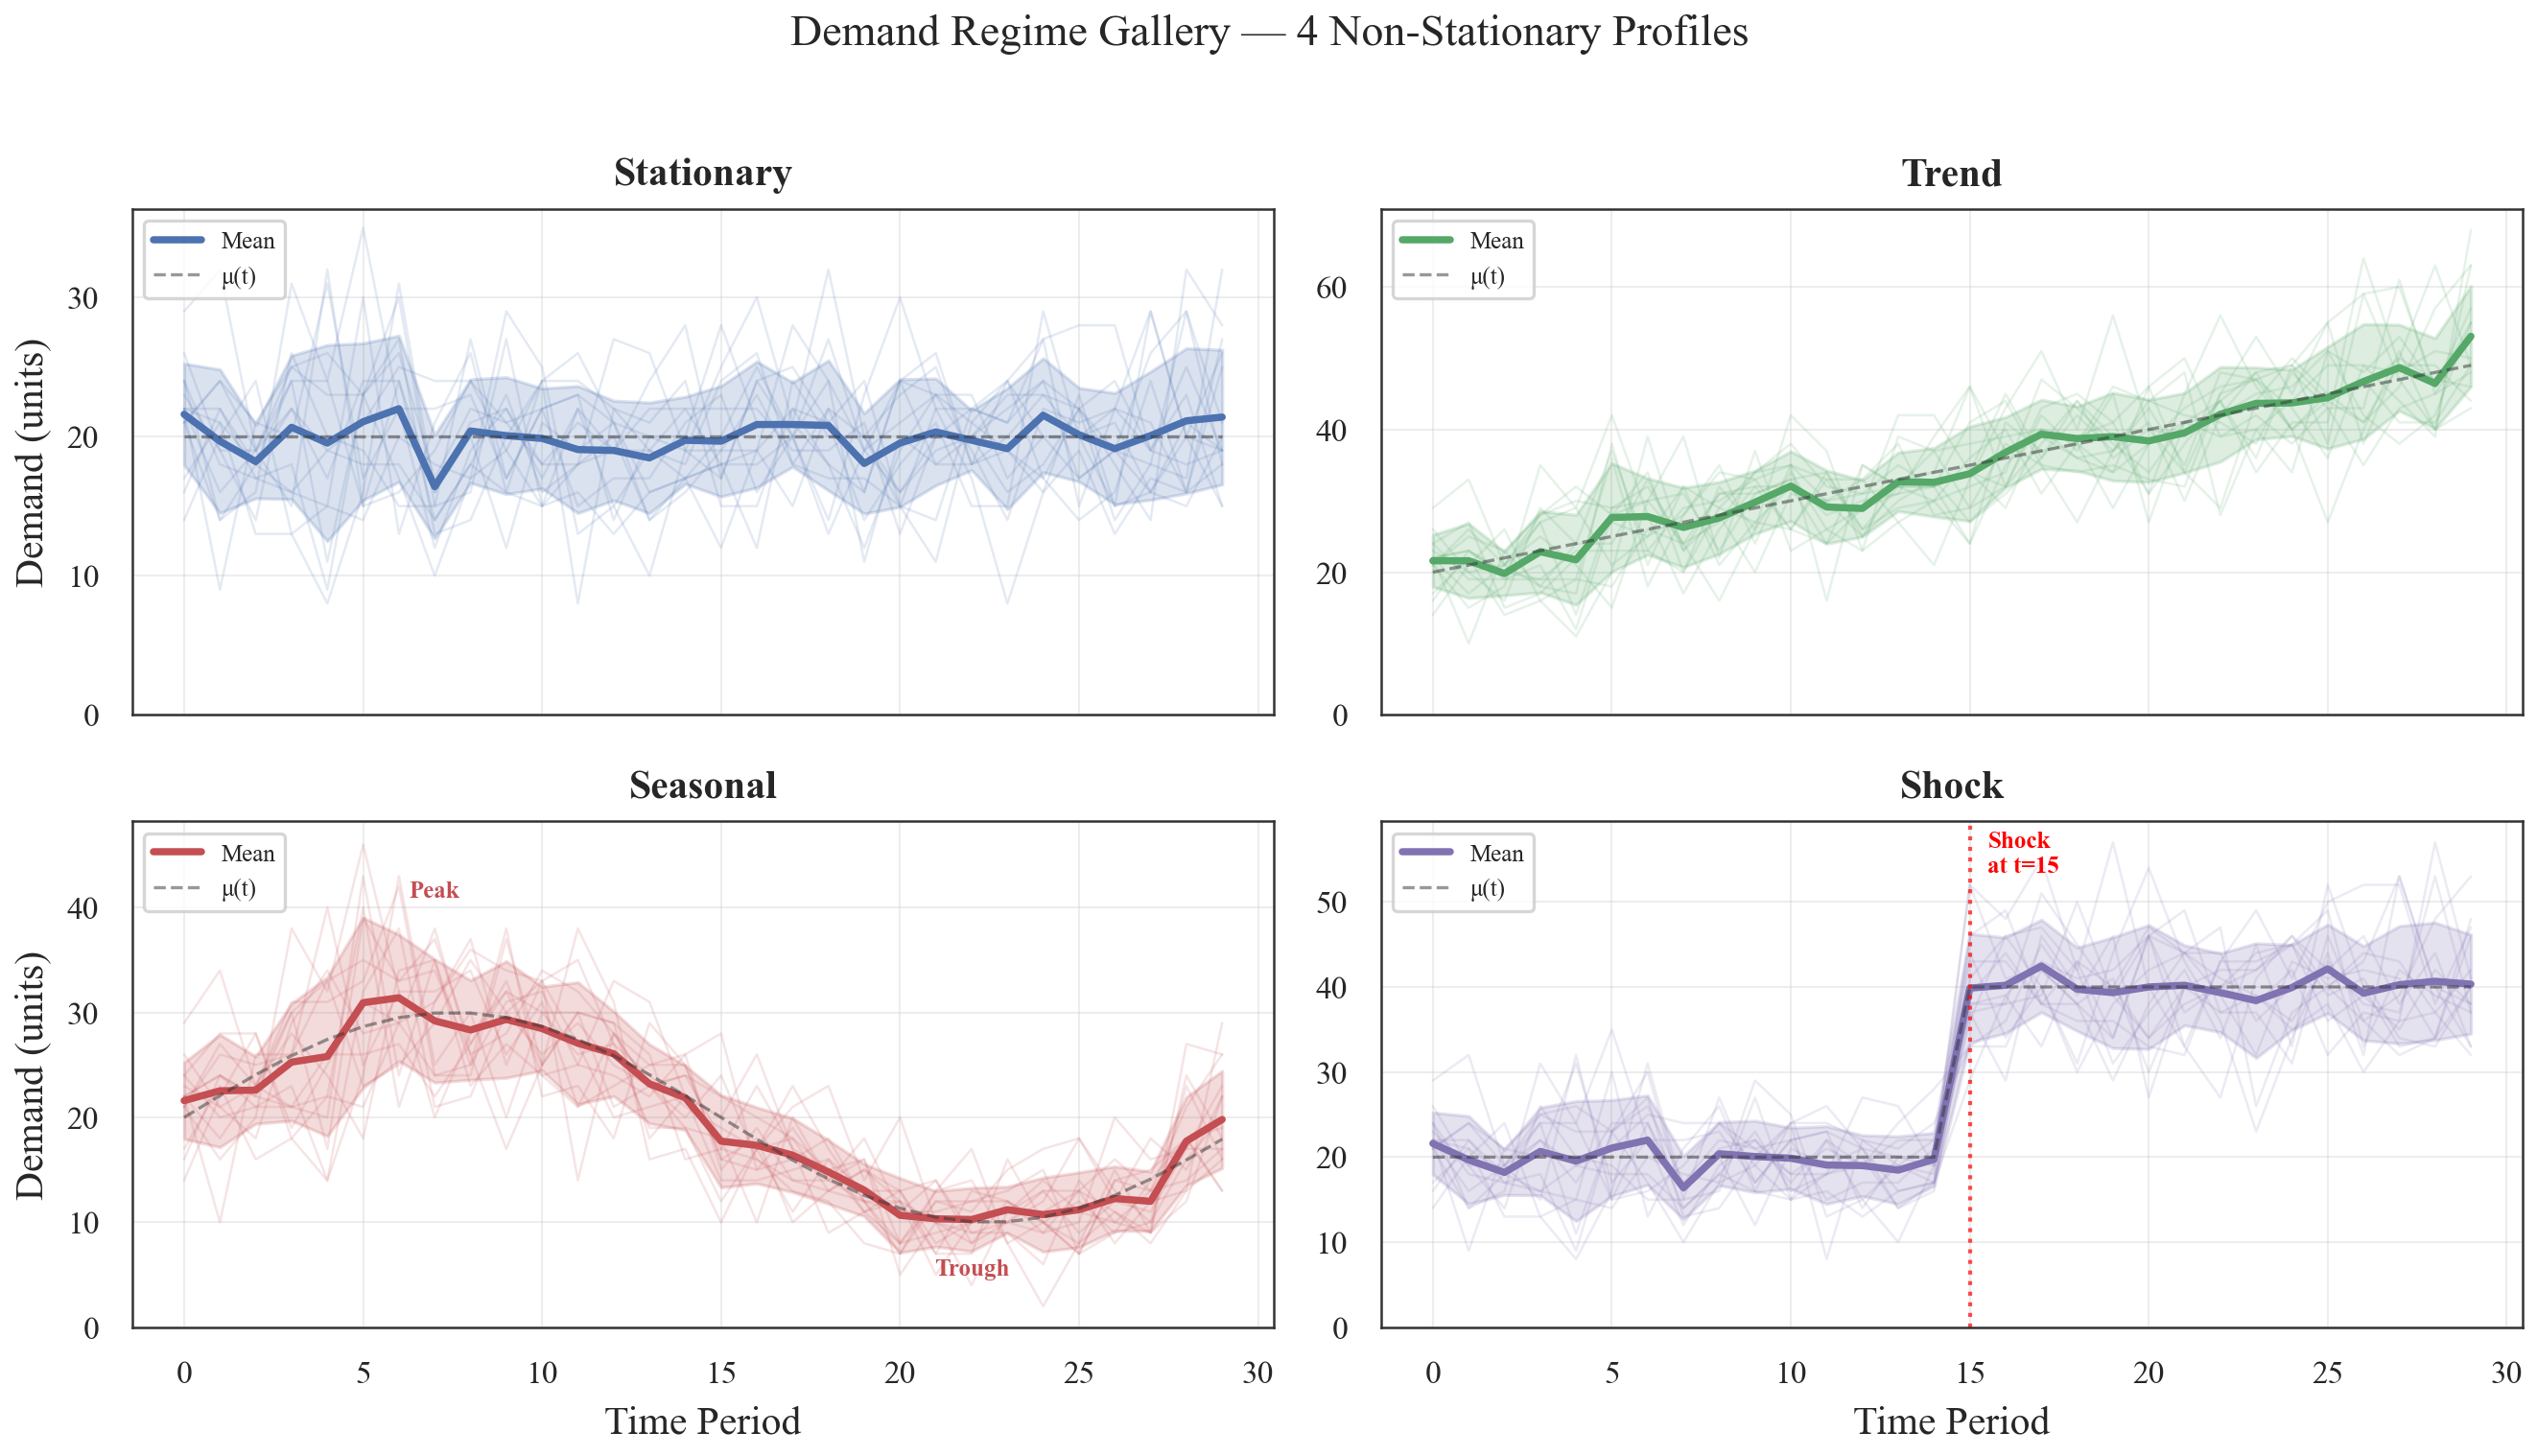
\includegraphics[width=0.9\textwidth]{figures/E1_demand_profile_gallery.png}
  \caption{Demand profile gallery showing the four base patterns over
           one 30-period episode. Shaded regions indicate $\pm 1$
           standard deviation of the Poisson draw. The shock pattern
           (bottom right) represents the most challenging setting for
           methods that assume distributional stationarity.}
  \label{fig:demand_gallery}
\end{figure}

\subsection{Operational Modes}

Each scenario is further characterized by two binary operational flags
that substantially alter the problem dynamics:

\paragraph{Goodwill (Endogenous Demand Feedback).}
When enabled, customer sentiment $\sigma_t \in
[\sigma_{\text{floor}}, \sigma_{\text{cap}}] = [0.2, 2.0]$ evolves
based on fulfillment quality:
\begin{equation}\label{eq:goodwill}
  \sigma_{t+1} = \begin{cases}
    \min(\sigma_{\text{cap}},\; \sigma_t \cdot g^+) & \text{if } U_t = 0
    \quad (g^+ = 1.01), \\
    \max(\sigma_{\text{floor}},\; \sigma_t \cdot g^-) & \text{if } U_t > 0
    \quad (g^- = 0.90),
  \end{cases}
\end{equation}
where $U_t$ is unfulfilled demand. The effective demand mean becomes
$\mu_t^{\text{eff}} = \sigma_t \cdot \mu_t$, creating an endogenous
feedback loop: a single stock-out triggers a 10\% sentiment drop,
while perfect service yields only 1\% growth---an asymmetric penalty
designed to model the well-documented phenomenon that customer
dissatisfaction propagates faster than satisfaction.

Goodwill scenarios are particularly important for benchmarking because
they \textbf{violate the exogenous-demand assumption} that underpins
most classical OR formulations (MSSP, DLP, newsvendor). This creates
a natural testbed for evaluating whether learning-based methods, which
can implicitly capture feedback dynamics from experience, offer an
advantage over optimization-based approaches that cannot model
endogenous demand.

\paragraph{Backlog vs.\ Lost Sales.}
When backlog is enabled, unfulfilled demand is carried over to the
next period with an associated penalty cost; otherwise, unfulfilled
demand is permanently lost. This binary flag alters the cost structure
and the feasibility of ``catch-up'' strategies after stock-outs.

\subsection{Observation and Action Spaces}

At each period~$t$, the agent observes a vector containing:
\begin{itemize}
  \item On-hand inventory $X_t^n$ for each node~$n$,
  \item Pipeline inventory $Y_t^e$ for each edge~$e$ (units in transit
        at each lead-time stage),
  \item Backlog $B_t^n$ (if applicable),
  \item Demand history $D_{t-k:t}$ (configurable lookback window,
        default $k = 5$).
\end{itemize}

We distinguish two information structures:
\begin{itemize}
  \item \textbf{Informed agents} have access to the true demand
        distribution parameters ($\mu_t$, pattern type). This models
        the idealized case where the planner has perfect knowledge of
        the demand-generating process.
  \item \textbf{Blind agents} must estimate demand parameters from
        the observed demand history alone. This models the realistic
        case where the demand process is unknown and must be learned.
\end{itemize}

The action space is $\mathcal{A} = \RR_{\geq 0}^{|\mathcal{E}|}$:
a continuous replenishment quantity for each edge in the supply chain
graph. Actions are clipped by the environment to respect available
upstream inventory and capacity constraints, ensuring physical
feasibility.

\subsection{Reward Structure}

The per-period reward is the \emph{net profit}:
\begin{equation}\label{eq:reward}
  r_t = \underbrace{\sum_{(i,j) \in \mathcal{E}_r} p_j \cdot S_t^{(i,j)}}
          _{\text{revenue}}
      - \underbrace{\sum_{n \in \mathcal{N}} h_n \cdot X_t^n}
          _{\text{holding cost}}
      - \underbrace{\sum_{(i,j) \in \mathcal{E}} g_{ij} \cdot Y_t^{(i,j)}}
          _{\text{pipeline cost}}
      - \underbrace{\sum_{n \in \mathcal{N}_r} b_n \cdot U_t^n}
          _{\text{backlog/lost cost}},
\end{equation}
where $S_t^{(i,j)}$ is the quantity sold on edge $(i,j)$, $U_t^n$ is
unfulfilled demand at retail node~$n$, and $b_n$ is the backlog or
lost-sales penalty. The total episode profit
$\Pi = \sum_{t=0}^{T-1} r_t$ (with $T = 30$ periods) serves as the
primary performance metric for all agents.

This reward structure is consistent across all solution methods:
classical OR agents (Oracle, MSSP, DLP, heuristics) and learning-based
agents (RL, GNN) are all evaluated using the same profit calculation
on the same environment transitions, ensuring a fair comparison.
\Cref{fig:reward_decomp} illustrates a representative reward
decomposition for the base network under stationary demand.

\begin{figure}[htbp]
  \centering
  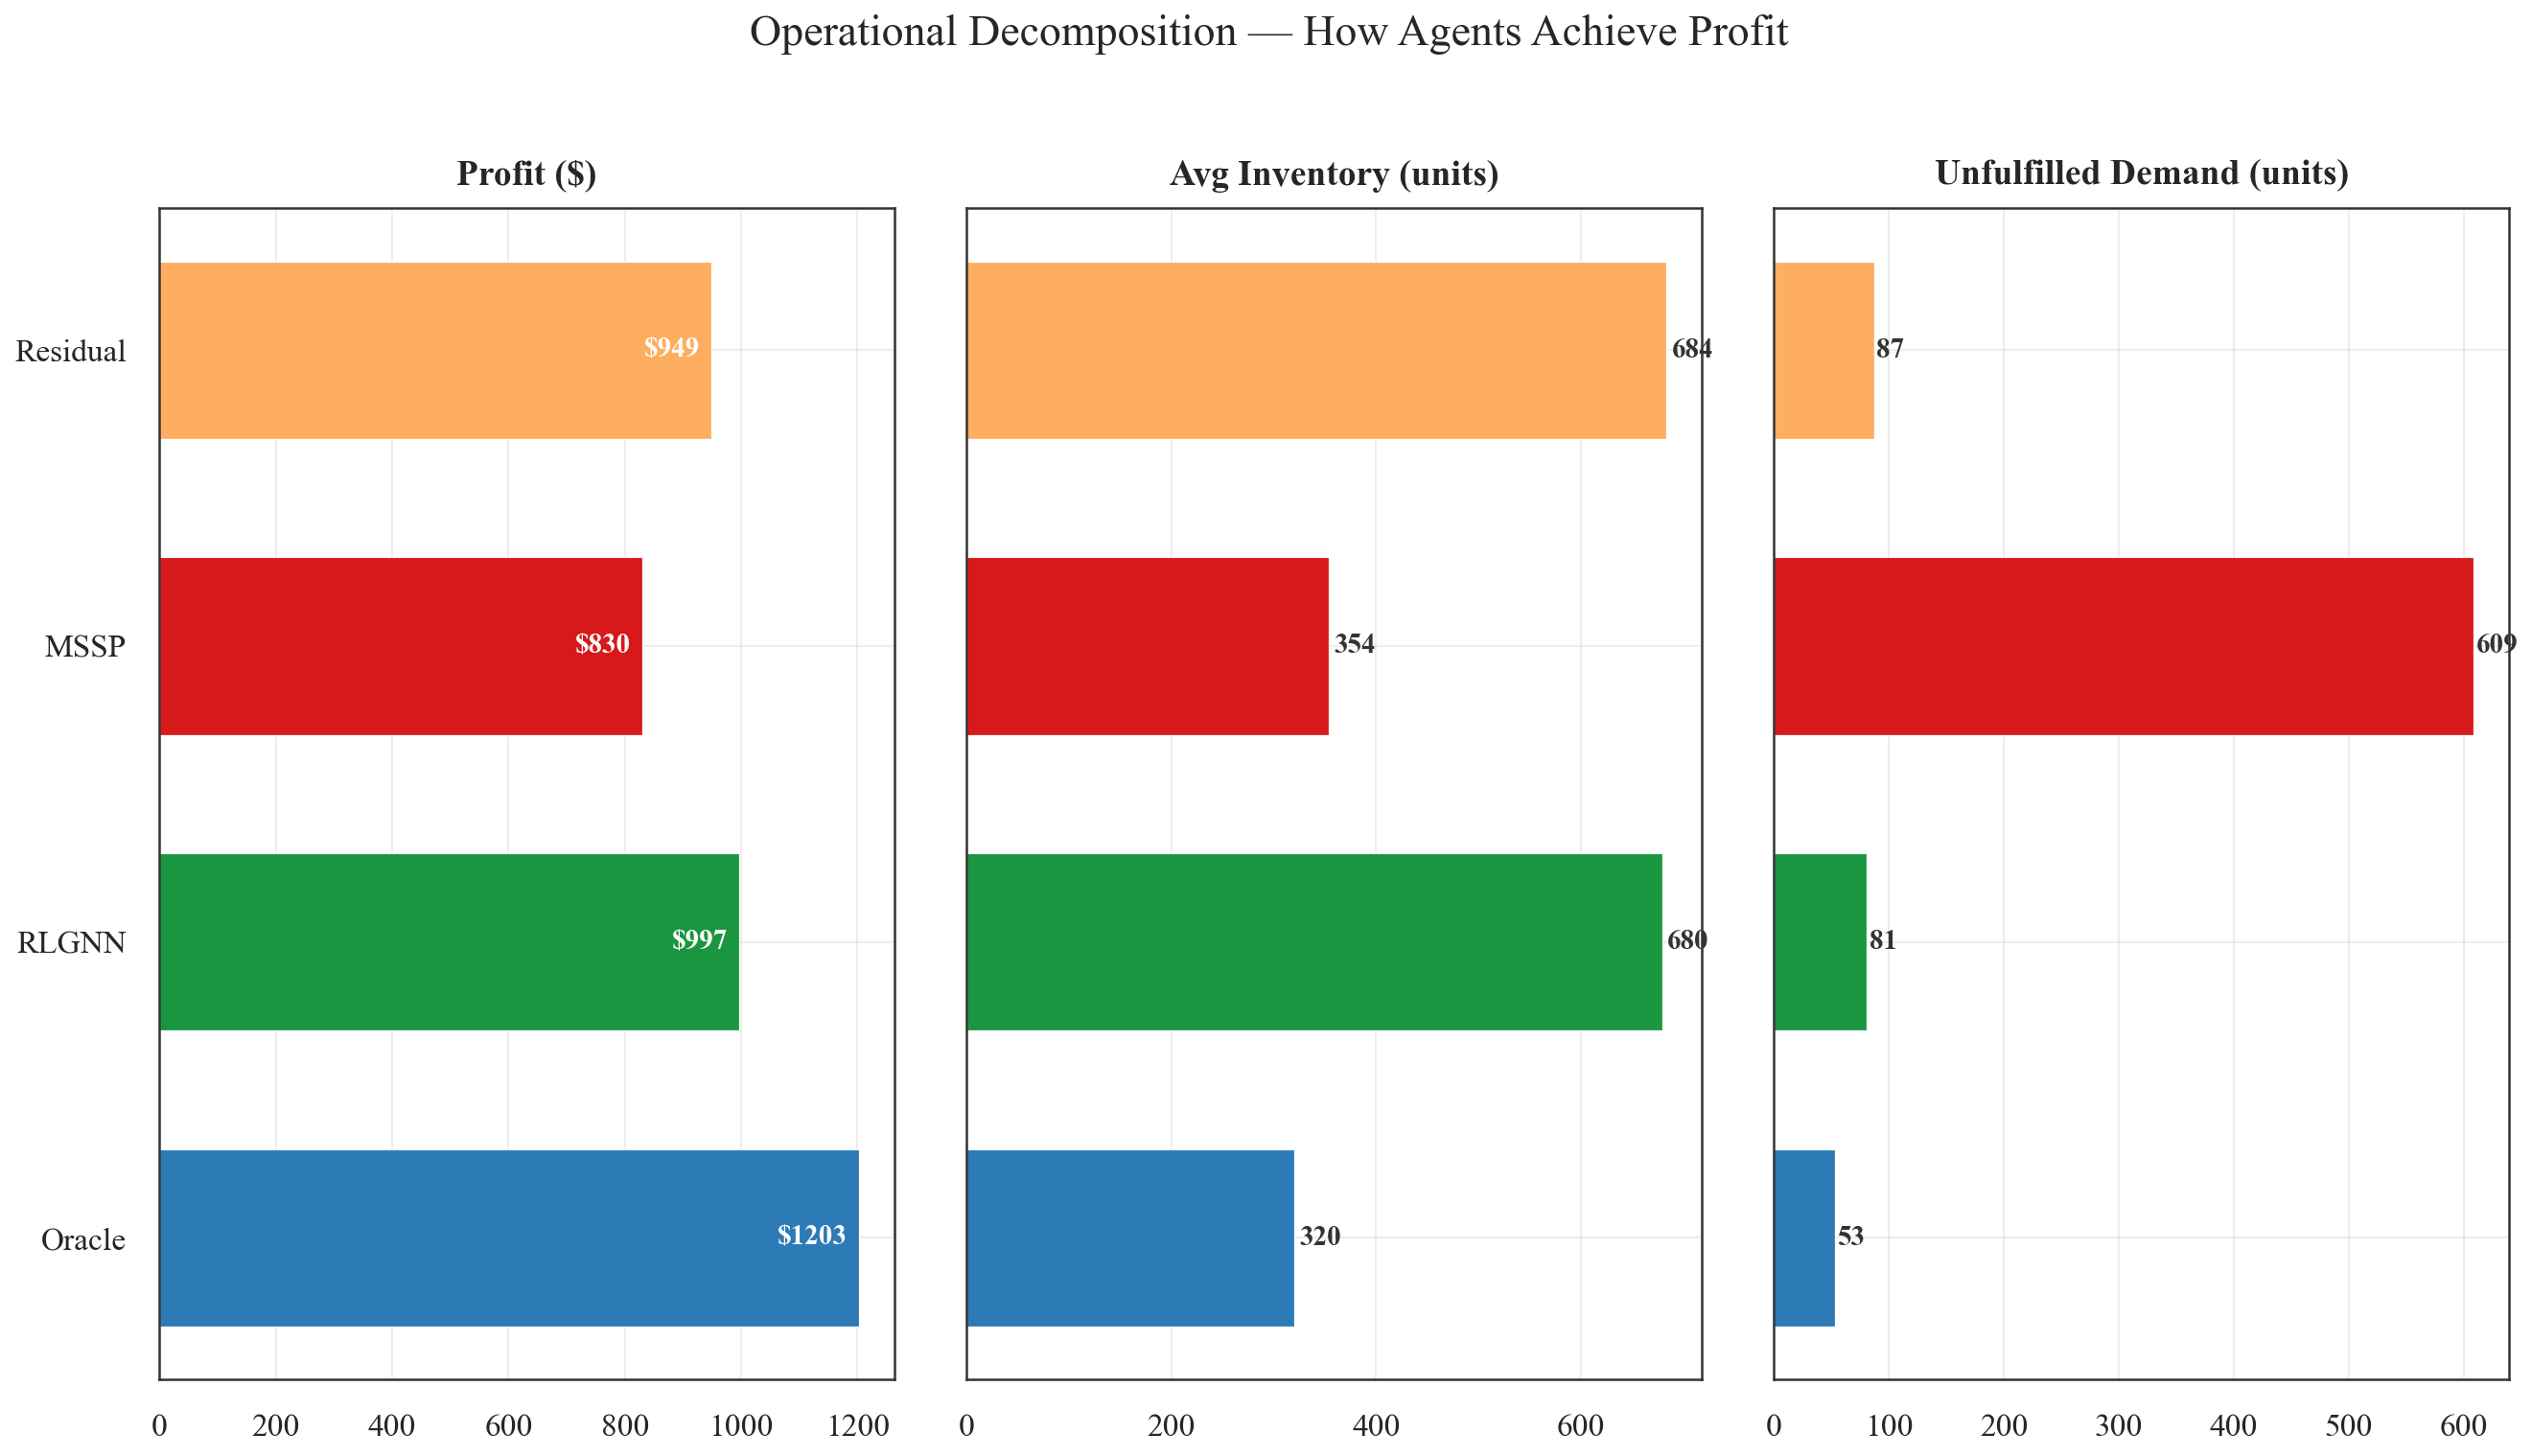
\includegraphics[width=0.85\textwidth]{figures/E4_reward_decomposition.png}
  \caption{Reward decomposition showing the per-period breakdown of
           revenue, holding cost, pipeline cost, and backlog/lost-sales
           penalty for the base network under stationary demand. The
           net profit (bold line) is the algebraic sum of all
           components.}
  \label{fig:reward_decomp}
\end{figure}

\subsection{Scenario Matrix}

By combining the dimensions described above, we construct a systematic
$2 \times 4 \times 2 \times 2 = 32$ scenario matrix
(\Cref{tab:scenarios}). Each scenario is uniquely identified by its
configuration of (network topology, demand pattern, goodwill mode,
backlog mode).

\begin{table}[htbp]
\centering
\caption{Scenario matrix: 32 configurations. Each row represents a
         unique combination of topology, demand, goodwill, and
         backlog settings.}
\label{tab:scenarios}
\small
\begin{tabular}{lcccc}
\toprule
\textbf{Network} & \textbf{Demand} & \textbf{Goodwill} & \textbf{Backlog}
                  & \textbf{Scenario ID} \\
\midrule
\multirow{8}{*}{Base}   & Stationary & \xmark & \cmark & B-St-NG-BL \\
                         & Stationary & \xmark & \xmark & B-St-NG-LS \\
                         & Trend      & \xmark & \cmark & B-Tr-NG-BL \\
                         & Trend      & \xmark & \xmark & B-Tr-NG-LS \\
                         & Seasonal   & \xmark & \cmark & B-Se-NG-BL \\
                         & Seasonal   & \xmark & \xmark & B-Se-NG-LS \\
                         & Shock      & \xmark & \cmark & B-Sh-NG-BL \\
                         & Shock      & \xmark & \xmark & B-Sh-NG-LS \\
\midrule
\multicolumn{5}{c}{\emph{Same 8 patterns repeated with Goodwill = \cmark
                    (16 total for Base)}} \\
\midrule
\multicolumn{5}{c}{\emph{Same 16 patterns repeated for Serial network
                    (32 total)}} \\
\bottomrule
\end{tabular}
\end{table}

This systematic design enables controlled analysis: by comparing
results across rows, we isolate the effect of individual factors
(e.g., demand pattern) while holding all others constant. This is
the kind of controlled experimental design that has been difficult
to achieve in prior work, where each study uses a unique environment
configuration.
